\documentclass[letter]{book}

%%%%%% Import Package %%%%%%
\usepackage{graphicx}
\usepackage[unicode]{hyperref}
\usepackage{cite}
\usepackage{indentfirst}
\usepackage{multirow}
\usepackage{indentfirst}
\usepackage{titlesec}
\usepackage{xcolor}
\usepackage{listings}
\usepackage{fontspec,xunicode,xltxtra}
\usepackage{xeCJK}
\usepackage{hyperref}
\usepackage{enumerate}
\usepackage{epigraph}
\usepackage{amsmath}
\usepackage[xindy]{glossaries}
\usepackage{fancyhdr}
\usepackage{amsmath}
%\usepackage{TikZ}
\usepackage{ifthen}
\usepackage{longtable}

%%%% 下面的命令设置行间距与段落间距 %%%%
\linespread{1.4}
% \setlength{\parskip}{1ex}
\setlength{\parskip}{0.5\baselineskip}

%Set Code Format%
\lstloadlanguages{C, csh, make,python,Java}
\lstset{	  
	alsolanguage= XML,  
	tabsize=4, %  
	frame=shadowbox, %把代码用带有阴影的框圈起来  
	commentstyle=\color{red!50!green!50!blue!50},%浅灰色的注释  
	rulesepcolor=\color{red!20!green!20!blue!20},%代码块边框为淡青色  
	keywordstyle=\color{blue!90}\bfseries, %代码关键字的颜色为蓝色,粗体  
	showstringspaces=false,%不显示代码字符串中间的空格标记  
	stringstyle=\ttfamily, % 代码字符串的特殊格式  
	keepspaces=true, %  
	breakindent=22pt, %  
	numbers=left,%左侧显示行号 往左靠,还可以为right,或none,即不加行号  
	stepnumber=1,%若设置为2,则显示行号为1,3,5,即stepnumber为公差,默认stepnumber=1  
	%numberstyle=\tiny, %行号字体用小号  
	numberstyle={\color[RGB]{0,192,192}\tiny} ,%设置行号的大小,大小有tiny,scriptsize,footnotesize,small,normalsize,large等  
	numbersep=8pt,  %设置行号与代码的距离,默认是5pt  
	basicstyle=\footnotesize, % 这句设置代码的大小  
	showspaces=false, %  
	flexiblecolumns=true, %  
	breaklines=true, %对过长的代码自动换行  
	breakautoindent=true,%  
	breakindent=4em, %  	   
	aboveskip=1em, %代码块边框  
	tabsize=4,  
	showstringspaces=false, %不显示字符串中的空格  
	backgroundcolor=\color[RGB]{245,245,244},   %代码背景色  
	%backgroundcolor=\color[rgb]{0.91,0.91,0.91}    %添加背景色  
	escapeinside=``,  %在``里显示中文  
	%% added by http://bbs.ctex.org/viewthread.php?tid=53451  
	fontadjust,  
	captionpos=t,  
	framextopmargin=2pt,framexbottommargin=2pt,abovecaptionskip=-3pt,belowcaptionskip=3pt,  
	xleftmargin=4em,xrightmargin=4em, % 设定listing左右的空白  
	texcl=true
}

\graphicspath{{./Image/common/}{./Image/Api/}{./Image/InterfaceDesign/}{./Image/Attachment/}}

\begin{document}


\begin{titlepage}

\begin{center}


% Upper part of the page

\includegraphics[width=0.15\textwidth]{./logo}\\[1cm]    

\textsc{\LARGE University of Beer}\\[1.5cm]

\textsc{\Large Final year project}\\[0.5cm]


% Title
%\rule{3mm}{.1pt}
\hrule[1.5cm]


\hrule[1mm]{5mm}%


{ \huge \bfseries Lager brewing techniques}\\[0.4cm]

%\HRule \\[1.5cm]

% Author and supervisor
\begin{minipage}{0.4\textwidth}
\begin{flushleft} \large
\emph{Author:}\\
John \textsc{Smith}
\end{flushleft}
\end{minipage}
\begin{minipage}{0.4\textwidth}
\begin{flushright} \large
\emph{Supervisor:} \\
Dr.~Mark \textsc{Brown}
\end{flushright}
\end{minipage}

\vfill

% Bottom of the page
{\large \today}

\end{center}

\end{titlepage}

\part{Framework}


\section*{Spring}

http://stackoverflow.com/questions/31045955/using-configurationproperties-to-fill-map-in-generic-way

\subsection*{JDBC数据库重连}

在数据库重启后,程序无法重新连接到数据库。程序使用的是Hikari,找到了如下属性:

\begin{lstlisting}[language=Bash]
# 使用Hikari pool时,是否允许连接池暂停,默认为: false
spring.datasource.allow-pool-suspension=true
\end{lstlisting}

可以将连接池到c3p0,c3p0连接池本身具有数据库重连机制。目前常见到连接池如下表所示:

\begin{tabular}{|c|c|c|p{8cm}|c|}
	\hline
	\multirow{1}{*}{序号}
	& \multicolumn{1}{c|}{名称}  
	& \multicolumn{1}{c|}{协议} 
	& \multicolumn{1}{c|}{备注}\\			
	\cline{1-4}
	1 & c3p0 &  LGPL v.2.1  & C3P0是一个开源数据连接池,Hibernate3.0默认自带的数据连接池,性能比较稳定。\\
	\hline
	2 & HikariCP & Apache 2.0 & Fast, simple, reliable. HikariCP is a "zero-overhead" production ready JDBC connection pool. At roughly 130Kb, the library is very light. \\
	\hline
	3 & Druid & Apache 2.0 & Druid是Java语言中最好的数据库连接池。Druid能够提供强大的监控和扩展功能。 \\
	\hline
	4 & DBCP & Apache 2.0 & DBCP(DataBase connection pool),是 apache 上的一个 java 连接池项目,也是 tomcat 使用的连接池组件。单独使用dbcp需要2个包:commons-dbcp.jar,commons-pool.jar \\
	\hline
	5 & BoneCP & Apache 2.0 & 使用HikariCP替代\\
	\hline
\end{tabular}

登陆服务器,使用命令查看正常的数据库连接:

\begin{lstlisting}[language=Bash]
lsof -i:5236
\end{lstlisting}

输出的结果如下:

\begin{lstlisting}
COMMAND   PID USER   FD   TYPE  DEVICE SIZE/OFF NODE NAME
java    20026   hl   38u  IPv4 2197171      0t0  TCP localhost:58220->localhost:padl2sim (ESTABLISHED)
java    20026   hl   42u  IPv4 2197527      0t0  TCP localhost:58222->localhost:padl2sim (ESTABLISHED)
java    20026   hl   43u  IPv4 2197176      0t0  TCP localhost:58224->localhost:padl2sim (ESTABLISHED)
java    20026   hl   44u  IPv4 2197177      0t0  TCP localhost:58226->localhost:padl2sim (ESTABLISHED)
java    20026   hl   45u  IPv4 2197178      0t0  TCP localhost:58228->localhost:padl2sim (ESTABLISHED)
java    20026   hl   46u  IPv4 2197179      0t0  TCP localhost:58230->localhost:padl2sim (ESTABLISHED)
java    20026   hl   47u  IPv4 2197180      0t0  TCP localhost:58232->localhost:padl2sim (ESTABLISHED)
java    20026   hl   48u  IPv4 2197181      0t0  TCP localhost:58234->localhost:padl2sim (ESTABLISHED)
java    20026   hl   49u  IPv4 2197182      0t0  TCP localhost:58236->localhost:padl2sim (ESTABLISHED)
java    20026   hl   50u  IPv4 2197536      0t0  TCP localhost:58238->localhost:padl2sim (ESTABLISHED)
\end{lstlisting}

在程序启动时,并没有真正建立TCP连接。只有真正的接受到请求查询数据库时,程序才与数据库建立TCP连接。此处建立了10个TCP连接。而Hikari默认的最大连接池数量也为10个。如下配置设启连接池连接池时,初始建立的连接数量为5个:

\begin{lstlisting}
spring.datasource.initial-size=5
\end{lstlisting}

在Spring中配置数据源类型如下:

\begin{lstlisting}
# 指定数据源类型
spring.datasource.type=com.zaxxer.hikari.HikariDataSource
\end{lstlisting}

Hikari默认的数据源默认的连接池数量为10个,默认的数量在HikariConfig类中进行的设置。为什么修改Spring的Initial Size数量会影响Hikari的连接数量呢?如果不配置数据源,Spring Boot默认的数据源是:

\begin{lstlisting}
org.apache.tomcat.jdbc.pool.DataSource
\end{lstlisting}

但是在实际开发中,可能需要使用自己是熟悉的数据源或者其他性能比较高的数据源。此时就可以通过制定Spring的数据源类型来实现。

停止数据库:

\begin{lstlisting}[language=Bash]
nohup sudo /opt/dmdbms/bin/dmserver /opt/dmdbms/data/DAMENG/dm.ini -noconsole &
\end{lstlisting}

在反复研究后发现,程序并未使用HikariCP连接池,而是使用的Spring JDBC连接池,所以在初始化Datasource时指定连接池,如下代码片段所示:

\begin{lstlisting}[language=Java]
@Configuration
@Data
@ConfigurationProperties(prefix = "spring.datasource")
public class DataSourceConfig {

	private String jdbcUrl;
	
	private String username;
	
	private String driverClassName;
	
	private String password;
	
	@Bean
	@Primary
	public DataSource primaryDataSource() {
		HikariConfig hikariConfig = new HikariConfig();
		hikariConfig.setDriverClassName(driverClassName);
		hikariConfig.setJdbcUrl(jdbcUrl);
		hikariConfig.setUsername(username);
		hikariConfig.setPassword(password);
		hikariConfig.setMaximumPoolSize(5);
		hikariConfig.setConnectionTestQuery("SELECT 1");
		hikariConfig.setPoolName("springHikariCP");
		hikariConfig.addDataSourceProperty("dataSource.cachePrepStmts", "true");
		hikariConfig.addDataSourceProperty("dataSource.prepStmtCacheSize", "250");
		hikariConfig.addDataSourceProperty("dataSource.prepStmtCacheSqlLimit", "2048");
		hikariConfig.addDataSourceProperty("dataSource.useServerPrepStmts", "true");
		HikariDataSource dataSource = new HikariDataSource(hikariConfig);
		return dataSource;
	}
}
\end{lstlisting}

\subsection{读取properties属性}

\subsubsection{读取自定义属性}

有时需要读取自定义属性,以配置HikariCP连接池为例,在application.properties文件指定指定配置:

\begin{lstlisting}
spring.datasource.hikari.jdbc-url=jdbc:dm://dn4:5236/DMSERVER
\end{lstlisting}

在类中获取配置相应的值,注意需要添加Data注解,否则需要手写get和set方法:

\begin{lstlisting}[language=Java]
@Configuration
@Data
@ConfigurationProperties(prefix = "spring.datasource.hikari")
public class DataSourceConfig {
	private String jdbcUrl;
}
\end{lstlisting}

由于此处注解是默认写在application.properties配置文件中,所以在ConfigurationProperties中可以不指定路径。否则需要使用locations指定配置文件路径。

\subsection{jps}

jps(Java Virtual Machine Process Status Tool)是JDK 1.5提供的一个显示当前所有java进程pid的命令。jdk中的jps命令可以显示当前运行的java进程以及相关参数,它的实现机制如下:

java程序在启动以后,会在java.io.tmpdir指定的目录下,就是临时文件夹里,生成一个类似于hsperfdata\_User的文件夹,这个文件夹里(在Linux中为/tmp/hsperfdata\_\{userName\}/),有几个文件,名字就是java进程的pid,因此列出当前运行的java进程,只是把这个目录里的文件名列一下而已。 至于系统的参数什么,就可以解析这几个文件获得。hsperfdata的含义就是HotSpot Performance Data。

\begin{lstlisting}[language=Bash]
nohup java -jar -Xmx2g credit-system-web-boot-1.0.0.jar --spring.config.location=application-jenkins.properties &
\end{lstlisting}


\newpage
\section*{Groovy}

\part{Tool}

\newpage

\section{OS}

\subsection{Linux}

\subsubsection{查看Linux信息}

\begin{lstlisting}[language=Bash]
# Linux查看版本当前操作系统内核信息
uname -a 
\end{lstlisting}


\section*{Gradle}

\subsection{执行流程}

There is a one-to-one relationship between a Project and a "build.gradle" file. During build initialisation, Gradle assembles a Project object for each project which is to participate in the build, as follows:

Create a Settings instance for the build.
Evaluate the "settings.gradle" script, if present, against the Settings object to configure it.
Use the configured Settings object to create the hierarchy of Project instances.
Finally, evaluate each Project by executing its "build.gradle" file, if present, against the project. The projects are evaluated in breadth-wise order, such that a project is evaluated before its child projects. This order can be overridden by calling evaluationDependsOnChildren() or by adding an explicit evaluation dependency using evaluationDependsOn(String).

\subsection{repositories}

在Gradle构建标本build.gradle里,经常会看到如下脚本:

\begin{lstlisting}[language=Java]
repositories {
	maven {
		url 'http://www.eveoh.nl/files/maven2'
	}
	maven {
		url 'http://repox.gtan.com:8078'
	}
	mavenCentral()
	jcenter()
	maven { url 'http://repo.spring.io/plugins-release' }
}
\end{lstlisting}

总的来说,只有两个标准的Android library文件服务器:Jcenter 和 Maven Central。起初,Android Studio 选择Maven Central作为默认仓库。如果你使用老版本的Android Studio创建一个新项目,mavenCentral()会自动的定义在build.gradle中。但是Maven Central的最大问题是对开发者不够友好。上传library异常困难。上传上去的开发者都是某种程度的极客。同时还因为诸如安全方面的其他原因,Android Studio团队决定把默认的仓库替换成jcenter。正如你看到的,一旦使用最新版本的Android Studio创建一个项目,jcenter()自动被定义,而不是mavenCentral()。mavenCentral()表示依赖是从Central Maven 2 仓库中获取的,库的地址是\url{https://repo1.maven.org/maven2}。jcenter表示依赖是从Bintary’s JCenter Maven 仓库中获取的,仓库的地址是\url{https://jcenter.bintray.com},bintray是一家提供全球企业软件开发包托管的商业公司。

\subsection{属性(Properties)}

\subsubsection{Extra Properties}

extra属性一般用于定义常量,All extra properties\footnote{\url{https://docs.gradle.org/current/javadoc/org/gradle/api/Project.html\#extraproperties}} must be defined through the "ext" namespace. Once an extra property has been defined, it is available directly on the owning object (in the below case the Project, Task, and sub-projects respectively) and can be read and updated. Only the initial declaration that needs to be done via the namespace.

\begin{lstlisting}[language=Java]
buildscript {
	ext {
		springBootVersion = '1.4.5.RELEASE'
		jacksonVersion = '2.8.7'
		springfoxVersion = '2.6.1'
		poiVersion = "3.14"
		aspectjVersion = '1.7.4'
	}
}
\end{lstlisting}

Reading extra properties is done through the "ext" or through the owning object.


ext.isSnapshot = version.endsWith("-SNAPSHOT")
if (isSnapshot) {
	// do snapshot stuff
}

\subsection{同时连接内外网}

在工作中,有时需要同时连接封闭的网络和互联网,开发环境需要依赖封闭的内网,与远程的同事交流需要依赖互联网,而封闭的内网与互联网切换是一大痛点,不仅影响效率,同时也影响心情,宝贵的时间就在这样无意义的开关中白白浪费掉了。制造障碍很容易,清除障碍很艰难。

解决双网卡问题,既能保证内网访问的安全,又能避免频繁切换网卡带来的时间开销,可谓一举两得。一般的计算机有有线网卡,也有无线网卡。一般情况下要么使用有线网卡,要么使用无线网卡,在使用无线时,连接上了有线,因为有线网卡的优先级高,故此时仅有有线能够工作,无线网卡可连接但是无法传送数据。实现双网卡的基本思路是删除默认网关,配置各自的网关即可。

\subsubsection{Mac同时连内网外网}

输入如下命令查看Mac的所有网络连接方式:

\begin{lstlisting}[language=Bash]
networksetup -listallnetworkservices
\end{lstlisting}

输出的结果如下:

\begin{lstlisting}
An asterisk (*) denotes that a network service is disabled.
Apple USB Ethernet Adapter
Wi-Fi
Bluetooth PAN
Thunderbolt Bridge
\end{lstlisting}

可以看出Mac可以通过Wi-Fi联网,也可以通过USB有线联网。给指定的网络连接方式设定DNS服务器代码如下:

\begin{lstlisting}[language=Bash]
sudo networksetup -setdnsservers AirPort 192.168.10.200
\end{lstlisting}

清空DNS缓存代码如下:

\begin{lstlisting}[language=Bash]
dscacheutil –flushcache
\end{lstlisting}

输入如下命令查看MacBook的路由表:

\begin{lstlisting}[language=Bash]
netstat -nr
\end{lstlisting}

\subsubsection{Fedora同时连接内外网}

给有线网卡配置地址信息时,内网网卡不要加默认网关,外网网卡加默认网关,并查看无线网卡分配到的地址信息中是否有默认网关。在这里内网是有线网络,外网是无线网络。使用route命令查看默认路由,输出如图\ref{fig:routetable}所示:

\begin{figure}[htbp]
	\centering
	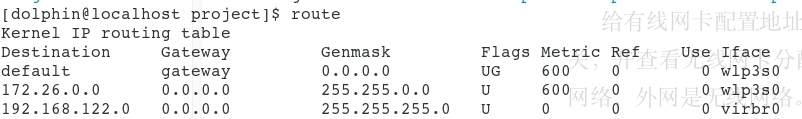
\includegraphics[scale=0.4]{route-table.jpg}
	\caption{查看Kernal路由表}
	\label{fig:routetable}
\end{figure}

其中wlp3s0是无线网卡的名称,说明此时的默认路由是无线网卡的路由。metric设置路由跳数,metric值越高,优先级越低。添加-p(permanent)参数永久保存此条路由信息,系统重启后路由也规则也不会丢失。三删除默认网关的命令如下:

\begin{lstlisting}[language=Bash]
sudo route del default
\end{lstlisting}

删除一条路由:

\begin{lstlisting}[language=Bash]
sudo route del -net 192.168.122.0 netmask 255.255.255.0
\end{lstlisting}

如果默认路由是外网网关。那么只需要单独为内网设置转发特例,所有59.214.*.*开头的,全部走enp0s26u1u2:

\begin{lstlisting}[language=Bash]
sudo route add -net 59.214.0.0 netmask 255.255.255.0 gw 10.55.10.1 dev enp0s26u1u2
\end{lstlisting}

其中59.214.0.0为内网IP的起始网段,255.255.0.0为内网的子网掩码,内网网关是10.36.40.12,eth0为内网网卡的名称。路由添加最好是添加到开机启动中:

\begin{lstlisting}[language=Bash]
vim /etc/rc.local
\end{lstlisting}

添加删除默认网关:

\begin{lstlisting}[language=Bash]
#添加默认网关
sudo route add default gw 10.55.10.1
#删除默认网关
sudo route del default gw 10.55.10.1
\end{lstlisting}

重启网络服务:

\begin{lstlisting}[language=Bash]
/etc/init.d/networking restart
\end{lstlisting}

此时可以同时访问互联网和局域网中的主机,但是无法访问A网络。访问A网络可通过局域网代理的方式访问,将局域网的一台主机作为代理服务器,本机访问局域网中的代理服务器,代理服务器再将请求转发给A网络。在本机只需要在浏览器中配置好代理服务器即可。以FireFox浏览器为例,在Preference->Advance->Network->Connection->Settings中,增加手动代理配置,地址填写代理主机的地址,端口填写8888,代理服务器运行的是Fiddler。以后,访问内网时就使用FireFox浏览器,访问外网时就使用Google Chrome浏览器。


\subsubsection{Ubuntu同时连接内外网}

\subsubsection{Windows同时连接内外网}

\url{http://blog.csdn.net/jay329106193/article/details/8129374}

\url{http://www.jianshu.com/p/b64da1d93e3d}



\section{Ansible}

\section{Fiddler}

\subsection{Fiddler替换Host}

\section{OpenVPN}

此处使用的OpenVPN版本是2.4.1。如果使用Mac下的brew工具安装,则OpenVPN目录在:/usr/local/Cellar/openvpn/2.4.1,OpenVPN的配置文件在:/usr/local/etc/openvpn。

\subsection{安装}

\subsubsection{生成客户端证书}

新建client文件夹,文件夹可随意命名,然后拷贝easy-ras文件夹到client文件夹,进入下列目录:

\begin{lstlisting}[language=Bash]
cp -R /etc/openvpn/easyrsa/ .
\end{lstlisting}

初始化:

\begin{lstlisting}[language=Bash]
./easyrsa init-pki.
\end{lstlisting}

服务端生成的文件有:

\begin{tabular}{|c|p{8cm}|c|}
	\hline
	\multirow{1}{*}{序号}
	& \multicolumn{1}{c|}{名称}  \\			
	\cline{1-2}
	ca.crt  & C3P0是一个开源数据连接池,Hibernate3.0默认自带的数据连接池,性能比较稳定。\\
	\hline
	reqs/server.req  & C3P0是一个开源数据连接池,Hibernate3.0默认自带的数据连接池,性能比较稳定。\\
	\hline
	reqs/dolphin.req  & C3P0是一个开源数据连接池,Hibernate3.0默认自带的数据连接池,性能比较稳定。\\
	\hline
	private/ca.key & \\
	\hline
	private/server.key & \\
	issued/server.crt & \\
	issued/dolphin.crt & \\
	dh.pem & \\
	\hline
\end{tabular}

客户端生成的文件有:

\begin{tabular}{|c|p{8cm}|c|}
	\hline
	\multirow{1}{*}{序号}
	& \multicolumn{1}{c|}{名称}  \\			
	\cline{1-2}
	private/dolphinclient.key  & C3P0是一个开源数据连接池,Hibernate3.0默认自带的数据连接池,性能比较稳定。\\
	\hline
	reqs/sdolphinclient.req & C3P0是一个开源数据连接池,Hibernate3.0默认自带的数据连接池,性能比较稳定。\\
	\hline
\end{tabular}

启动OpenVPN:

\begin{lstlisting}[language=Bash]
sudo openvpn server.conf
\end{lstlisting}

\subsection{常见错误}


\section{ssh}

\subsection{Session时间}

在使用ssh的过程中,经常会遇到一会儿没有操作就自动断开了,不是非常方便。

\paragraph{ClientAliveInterval}

修改/etc/ssh/sshd\_config配置文件 ClientAliveInterval 300(默认为0),参数的是意思是每5分钟,服务器向客户端发一个消息,用于保持连接,使用service sshd reload 让其修改后生效。如果发现还是有问题,可以试着把300设置小一点,例如60。

\paragraph{ClientAliveCountMax}

另外,至于ClientAliveCountMax, 使用默认值3即可.ClientAliveCountMax表示服务器发出请求后客户端没有响应的次数达到一定值, 就自动断开。

\paragraph{ControlPersist 4h}

在./ssh/config中添加一行:

\begin{lstlisting}[language=Bash]
ControlPersist 4h
\end{lstlisting}

When used in conjunction with ControlMaster, specifies that the master connection should remain open in the background (waiting for future client connections) after the initial client connection has been closed. If set to no, then the master connection will not be placed into the background, and will close as soon as the initial client connection is closed. If set to yes or 0, then the master connection will remain in the background indefinitely (until killed or closed via a mechanism such as the “ssh -O exit”). If set to a time in seconds, or a time in any of the formats documented in sshd\_config, then the backgrounded master connection will automatically terminate after it has remained idle (with no client connections) for the specified time\footnote{\url{http://man.openbsd.org/ssh_config.5}}.现在你每次通过SSH与服务器建立连接之后,这条连接将被保持4个小时,即使在你退出服务器之后,这条连接依然可以重用,因此,在你下一次(4小时之内)登录服务器时,你会发现连接以闪电般的速度建立完成,这个选项对于通过scp拷贝多个文件提速尤其明显,因为你不在需要为每个文件做单独的认证了。

\section{Curl}

\begin{lstlisting}[language=Bash]
curl 'http://59.214.215.6:3800/inapi/united/detail?param=%E8%B0%8A%E5%BE%B7%E5%AE%9E%E4%B8%9A&reds=&blacks=TS_F_HEIMINGDAN_C500033,TS_F_HEIMINGDAN' -H 'Pragma: no-cache' -H 'HL-APP-KEY: CreditChongqingSharePortal' -H 'DNT: 1' -H 'Accept-Encoding: gzip, deflate, sdch' -H 'Accept-Language: zh-CN,zh;q=0.8,en;q=0.6,zh-TW;q=0.4' -H 'User-Agent: Mozilla/5.0 (X11; Fedora; Linux x86_64) AppleWebKit/537.36 (KHTML, like Gecko) Chrome/55.0.2883.87 Safari/537.36' -H 'Accept: application/json, text/plain, */*' -H 'Cache-Control: no-cache' -H 'HL-CURRENT-URL: http://59.214.215.6:3800/main/search/unitedListQuery' -H 'Referer: http://59.214.215.6:3800/main/search/unitedListQuery' -H 'Cookie: UM_distinctid=15b667c97f65a-0afddd1bed9cb8-1421150f-15f900-15b667c97f737f; CNZZDATA1257579122=576897936-1492070602-http%253A%252F%252F59.214.215.6%253A8081%252F%7C1492393083; cc-o-t=ZnNoeEpnMXZUcklpRXAyTm9ReXhwWTdNSFFUMnptZ2NOdmFDWlhPajhlakRvYVk1eEtRem53enJMNVpzdU5HRURlejlRT3lqQ2VldHJUb2dETXZOVkIrcTZqZzR5M0xoUHZsL0V2TXZ1c3VYaVJkRE1NdEE5c0ZWMXI5dUVlV0g' -H 'Connection: keep-alive' --compressed
\end{lstlisting}

\section{Git}

\subsection{merge}

配置Meld为默认合并工具:

\begin{lstlisting}[language=Bash]
git config --global merge.tool meld
\end{lstlisting}



\section{LaTex}

\subsection{字体}

Computer Modern是自由软件TeX的默认字体,为美国计算机科学家高德纳(Donald Knuth)使用METAFONT软件创造。但是此字体不是很漂亮,所以考虑换一个字体 。


\part{Network}

\section{PAC}

\subsection{PAC简介}

PAC是proxy auto-config的缩写。PAC文件是纯文本格式的,实际上就是JavaScript文件。PAC最简单的格式就是包含一个叫FindProxyForURL的JavaScript函数,IE通过传入两个变量来调用这个函数。一个是用户流量的地址的URL全路径,一个是这个URL中的主机名host。在日常生活中浏览器中设置代理很简单,但是当你来回切换时总是觉得很烦,你可以使用pac脚本自动判断是否走代理,方便省去了来回手动切换的烦恼。

\subsection{PAC实例}

一个最简单的PAC脚本:

\begin{lstlisting}[language=VBScript]
function FindProxyForURL(url,host){
	return "DIRECT";
}
\end{lstlisting}

参数url是用户输入的url,参数host是url中的主机名。PAC文件返回值有三种类型:

\begin{itemize}
	\item{DIRECT直连不通过代理}
	\item{PROXY www.lybbn.cn:8080 http通过8080端口代理上网,也可以使用ip:port的形式}
	\item{SOCKS5 www.lybbn.cn:8080 socks通过8080端口代理上网,可以使用ip:port形式}
\end{itemize}

\begin{lstlisting}[language=VBScript]
var FindProxyForURL = function(init, profiles) {
	return function(url, host) {
		"use strict";
		var result = init, scheme = url.substr(0, url.indexOf(":"));
		do {
			result = profiles[result];
			if (typeof result === "function") result = result(url, host, scheme);
		} while (typeof result !== "string" || result.charCodeAt(0) === 43);
		return result;
	};
}("+dolphin2", {
	"+dolphin2": function(url, host, scheme) {
		"use strict";
		if (/^59\.214\.215\.6$/.test(host)) return "+dolphin-proxy";
		if (/^10\.10\.1\.11$/.test(host)) return "+dolphin-proxy";
		return "DIRECT";
	},
	"+dolphin-proxy": function(url, host, scheme) {
		"use strict";
		if (/^127\.0\.0\.1$/.test(host) || /^::1$/.test(host) || /^localhost$/.test(host)) return "DIRECT";
		return "PROXY 10.55.10.2:8888";
	}
});
\end{lstlisting}

以上脚本说明,当IP为59.214.215.6或10.10.1.11时,使用代理dolphin-proxy,而代理dolphin-proxy设置的是代理机器的相关信息,代理机器的IP为10.55.10.2,代理的端口是8888。

\end{document}
\theend
